\section{The Extracellular Matrix}

The extracellular matrix serves as more than just structural scaffolding for neural tissue. It forms an active component of the brain's information processing and energy management systems \cite{Dityatev2010}. This complex network of proteins, proteoglycans, and other molecules fills the space between cells, creating a structured environment that shapes both ionic flows and molecular signaling while providing crucial support for maintaining coherent states.

The interaction between astrocytic networks and the ECM proves particularly important for maintaining energetic coherence across subsystems \cite{Song2018}. The ECM creates organized diffusion pathways that guide the movement of ions and neurotransmitters through the extracellular space, helping regulate local signaling environments while supporting broader patterns of communication across neural tissue. This structured diffusion plays an essential role in shaping both synaptic transmission and volume transmission between cells \cite{Sykova2008}.

The molecular composition and organization of the ECM varies systematically across brain regions, reflecting local functional requirements and computational demands \cite{Bandtlow2000}. These regional specializations create distinct microenvironments that support different aspects of neural processing. Through specific arrangements of matrix proteins and proteoglycans, the ECM helps establish and maintain the precise conditions necessary for different forms of neural computation and state maintenance \cite{Zimmermann2008}.

Perineuronal nets, specialized ECM structures that surround specific neuronal subtypes, demonstrate particularly sophisticated organization \cite{Wang2012}. These nets stabilize synaptic connections while regulating local ion concentrations, enabling sustained high-frequency firing patterns in certain neural populations. The precise molecular composition of perineuronal nets helps create stable microenvironments that support reliable neural signaling while allowing for controlled plasticity \cite{Kwok2011}.

The broader interstitial matrix that fills the space between cells serves multiple crucial functions in neural processing \cite{Ruoslahti1996}. Beyond providing structural support, this matrix guides molecular diffusion, supports volume transmission, and helps maintain proper spacing between cellular elements \cite{Nicholson1998}. The physical properties of the interstitial matrix influence both local signaling dynamics and broader patterns of communication across neural tissue.

The dynamic interaction between cellular components and the ECM creates a structured environment that supports both stability and adaptability in neural processing \cite{Dityatev2003}. Rather than serving as a static scaffold, the ECM actively participates in shaping neural activity through its influence on molecular diffusion, ion distribution, and cellular communication. This dynamic role proves essential for maintaining the coherent states necessary for conscious processing.

\begin{figure}[h]
    \centering
    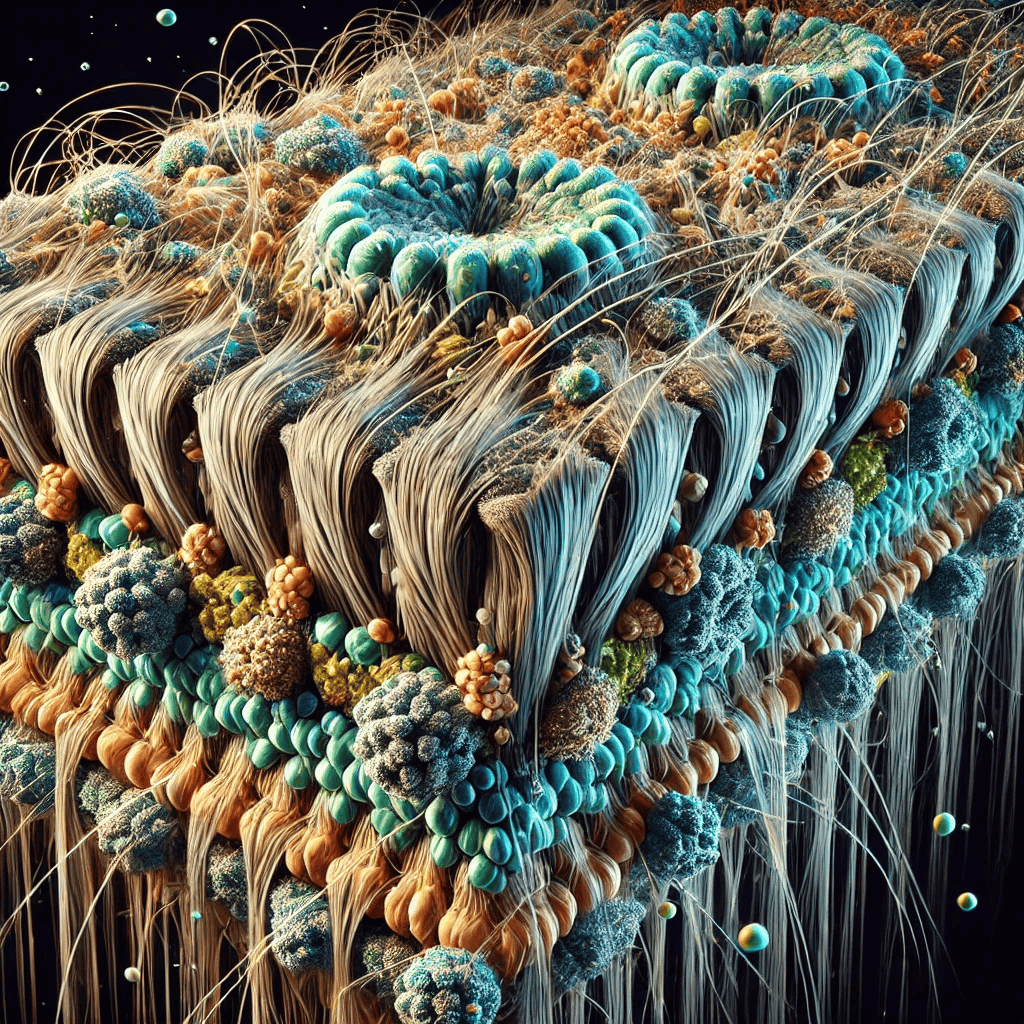
\includegraphics[width=0.8\textwidth]{ecm.png}

    \caption{The ECM guides ion flows and EM waves.}
\end{figure}

The ECM's influence on neural signaling extends beyond traditional synaptic transmission \cite{Vargova2014}. Through its capacity to bind and concentrate various signaling molecules, the matrix creates specialized signaling domains that shape both local and long-range communication. These domains help orchestrate complex patterns of neural activity while maintaining the stability necessary for coherent processing. The matrix's ability to sequester and release molecules in response to neural activity provides an additional layer of regulation in neural computation.

The relationship between the ECM and neural plasticity reveals sophisticated mechanisms for balancing stability and adaptability \cite{Dityatev2010}. While perineuronal nets help stabilize existing synaptic connections, local modifications of matrix composition can enable controlled reorganization of neural circuits \cite{Burnside2014}. This dynamic regulation of plasticity proves essential for learning and memory while maintaining the overall stability necessary for conscious processing.

Water and ion movement through the extracellular space depends critically on ECM organization \cite{Hrabetova2009}. The matrix creates structured pathways that guide fluid flow and ion diffusion, influencing both local signaling dynamics and broader patterns of neural activity. These pathways help maintain proper ionic balance while enabling efficient distribution of metabolites and removal of waste products. The resulting flow patterns support both local computation and global integration of neural activity.

The ECM's role in maintaining boundary conditions between different neural compartments deserves particular attention \cite{Barros2011}. Through specific molecular arrangements, the matrix helps establish and maintain distinct functional domains within neural tissue. These boundaries prove essential for proper circuit function while enabling controlled communication between different neural populations \cite{Frischknecht2012}. The precise organization of these boundary regions reflects evolutionary optimization for both isolation and integration of neural processing.

Matrix metalloproteinases and other ECM-modifying enzymes provide mechanisms for dynamic regulation of extracellular space properties \cite{Dityatev2003}. These enzymes can rapidly modify local matrix composition in response to neural activity, enabling adaptive changes in diffusion properties and signaling environments. This dynamic regulation allows neural circuits to adjust their processing capabilities while maintaining overall stability \cite{Song2018}.

The interaction between the ECM and glial cells represents another crucial aspect of neural organization \cite{Vargova2014}. Astrocytes actively participate in maintaining and modifying matrix composition, creating a feedback system that enables dynamic regulation of extracellular space properties. This interaction helps coordinate local changes in matrix structure with broader patterns of neural activity and metabolic demand.

The ECM's contribution to energetic coherence becomes particularly evident in its role in maintaining field effects across neural tissue \cite{Sykova2008}. The structured organization of matrix molecules influences the propagation of electromagnetic fields generated by neural activity, helping shape both local and global patterns of field interaction. This influence on field dynamics provides another mechanism through which the matrix contributes to conscious processing.

Understanding the ECM through ECC's framework reveals how seemingly passive structural elements can play active roles in consciousness \cite{Dityatev2010}. The matrix emerges not merely as a support system but as an essential component in maintaining the coherent energy states necessary for conscious experience. Its sophisticated molecular organization and dynamic properties enable both the stability required for reliable neural processing and the flexibility needed for adaptive responses \cite{Frischknecht2012}.

This deeper appreciation of the ECM's role suggests new approaches to both understanding and treating disorders of consciousness \cite{Burnside2014}. Matrix disruptions may contribute to various pathological conditions through their effects on neural signaling and energy coherence. Conversely, therapeutic interventions targeting matrix composition or organization might provide novel ways to influence conscious states and restore normal brain function.

The ECM's role extends beyond local circuit function to influence global brain dynamics \cite{Barros2011}. Through its effects on ion mobility, volume transmission, and field propagation, the matrix helps establish the conditions necessary for maintaining coherent states across multiple spatial scales. This multi-scale organization proves essential for understanding how consciousness emerges from coordinated neural activity \cite{Zimmermann2008}.

Having examined the biological components of neural tissue, we must now consider how to model the complex interactions within the neuropil that give rise to conscious states. This dense network of neural processes, glial cells, and extracellular matrix presents unique challenges for mathematical description and computational simulation.